\section{Обґрунтування вибору та налаштування середовища розробки}

\subsection{Аналіз інструментарію та обґрунтування вибору VS Code}

Згідно з методичними вказівками, для розробки програмного забезпечення на мові Java 
традиційно розглядається ``велика трійка'' інтегрованих середовищ розробки (IDE): NetBeans, 
Eclipse та IntelliJ IDEA. Проте в межах виконання даної лабораторної роботи було прийнято 
рішення відмовитися від стандартних автоматизованих майстрів генерації проектів на користь 
легковажного та універсального текстового редактора \textbf{Visual Studio Code (VS Code)}.

Такий підхід має низку суттєвих інженерних та освітніх переваг:
\begin{itemize}
    \item \textbf{Глибоке розуміння процесів компіляції:} 
    Використання автоматизованих систем збирання (Maven, Gradle) на початковому етапі приховує 
    від розробника внутрішні механізми взаємодії компілятора та віртуальної машини. Створення 
    проекту ``з нуля'' дозволяє повністю контролювати структуру каталогів та процес збирання 
    на рівні утиліт CLI.
    \item \textbf{Єдиний робочий простір (All-in-One):} 
    VS Code дозволяє об'єднати розробку вихідного коду мовою Java та верстку технічного 
    звіту (протоколу) в системі комп'ютерного набору \texttt{LaTeX} в межах одного вікна редактора.
    \item \textbf{Ефективність використання ресурсів:} На відміну від важких IDE, VS Code 
    має високу швидкість роботи та низькі вимоги до оперативної пам'яті, забезпечуючи при 
    цьому повноцінну підтримку мовного сервера Java.
\end{itemize}

\subsection{Встановлення програмного забезпечення та конфігурація системи}

Процес розгортання робочого оточення складався з наступних етапів:
\begin{enumerate}
    \item \textbf{Встановлення інструментарію Java:} 
    У систему було встановлено актуальний комплект розробника\\
     \texttt{Java Development Kit версії 27 (JDK-27)},
    який включає компілятор \texttt{javac} та виконавче середовище JVM.
    \item \textbf{Розширення VS Code:} 
    Для забезпечення інтелектуального аналізу коду (IntelliSense) та підсвічування синтаксису 
    в редактор було інтегровано офіційний пакет розширень \textit{Extension Pack for Java} від Microsoft.
    \item \textbf{Налаштування локалізації терміналу:} Для коректного відображення унікальних літер 
    українського алфавіту \textit{і}, \textit{ї}, \textit{є} у консолі Windows, сесію оболонки 
    було програмно переведено на роботу зі стандартом кодування \texttt{UTF-8}.
\end{enumerate}

\subsection{Автоматизація збирання та формування єдиного циклу розробки}

Для повної автоматизації рутинних операцій компіляції коду та генерації звіту було створено 
кастомний сценарій планувальника завдань всередині файлу \texttt{.vscode/tasks.json}. Облочкою виконання 
було обрано середовище Windows PowerShell.

Розроблена конфігурація об'єднує два послідовних процеси (Завдання) в один ультимативний цикл збирання:
\begin{enumerate}
    \item \textbf{Завдання компіляції та запуску Java:} 
    Компілює всі вихідні файли пакету за допомогою \texttt{javac} із примусовим прапорцем \texttt{-encoding UTF-8}, 
    зберігає бінарні файли \texttt{.class} у каталог \texttt{bin}, ініціалізує UTF-8 кодування консолі та запускає 
    віртуальну машину \texttt{java.exe} для виконання класу \texttt{Main}.
    \item \textbf{Завдання верстки звіту:} Переходить у каталог \texttt{report} та викликає компілятор \texttt{xelatex} 
    із прапорцем \texttt{-shell-escape} для генерації підсумкового PDF-документа, автоматично підтягуючи оновлені 
    лістинги коду.
\end{enumerate}

Завдяки такій конфігурації, натисканням однієї комбінації клавіш \texttt{Ctrl + Shift + B} виконується повний цикл: 
від перевірки працездатності алгоритмів Java до формування фінального друкованого протоколу лабораторної роботи.

\subsection{Реалізація концепції базового пакету та структури проєкту вручну}

Згідно з методичними вказівками, під час створення проєкту в IntelliJ IDEA особлива увага приділяється налаштуванню 
параметра \textbf{Base package} (базового пакету) у форматі \texttt{[назва\_групи].[прізвище]} (наприклад, \texttt{ad251.gorbunova})~\cite{1}. 
У мові Java концепція пакетів (\texttt{package}) виконує роль просторів імен і логічного групування класів, але її 
фундаментальною особливістю є те, що \textbf{структура пакетів в коді повинна строго відповідати фізичній структурі папок на диску}.

Під час кастомного налаштування проєкту у VS Code цей процес не приховувався за автоматичними майстрами IDE, 
а був реалізований повністю вручну за такими етапами:

\begin{enumerate}
    \item \textbf{Створення фізичної ієрархії каталогів:} 
    У корені робочого простору було створено каталог вихідного коду \texttt{src}, всередині якого вручную розгорнуто 
    ланцюжок папок, що точно відповідає структурі базового пакету: \texttt{src/ad251/gorbunova/}.
    \item \textbf{Конфігурація логічного кореня (Source Root):} 
    Для того щоб мовний сервер Java у VS Code коректно інтерпретував ієрархію, у файлі налаштувань 
    середовища \texttt{.vscode/settings.json} було явно вказано шлях до вихідних файлів за допомогою параметра:
    \begin{verbatim}
    "java.project.sourcePaths": ["src"]
    \end{verbatim}
    Завдяки цьому середовище починає відлік простору імен саме з папки \texttt{src}, 
    і шлях \texttt{src/ad251/gorbunova/Main.java} стає повністю еквівалентним 
    оголошенню \texttt{package ad251.gorbunova;} в першому рядку кожного файлу.
    \item \textbf{Ізоляція артефактів збирання:} 
    На відміну від стандартного підходу, де скомпільовані файли суміщаються з вихідним кодом, за допомогою 
    прапорця \texttt{-d bin} утиліти \texttt{javac} було налаштовано автоматичне дзеркальне створення структури 
    пакетів у відокремленому бінарному каталозі \texttt{bin/ad251/gorbunova/}.
\end{enumerate}

На рисунку~\ref{fig:project_tree} представлено фінальну архітектуру та дерево папок розробленого 
проєкту, згенероване безпосередньо в робочому просторі.

\begin{figure}[H]
    \centering
    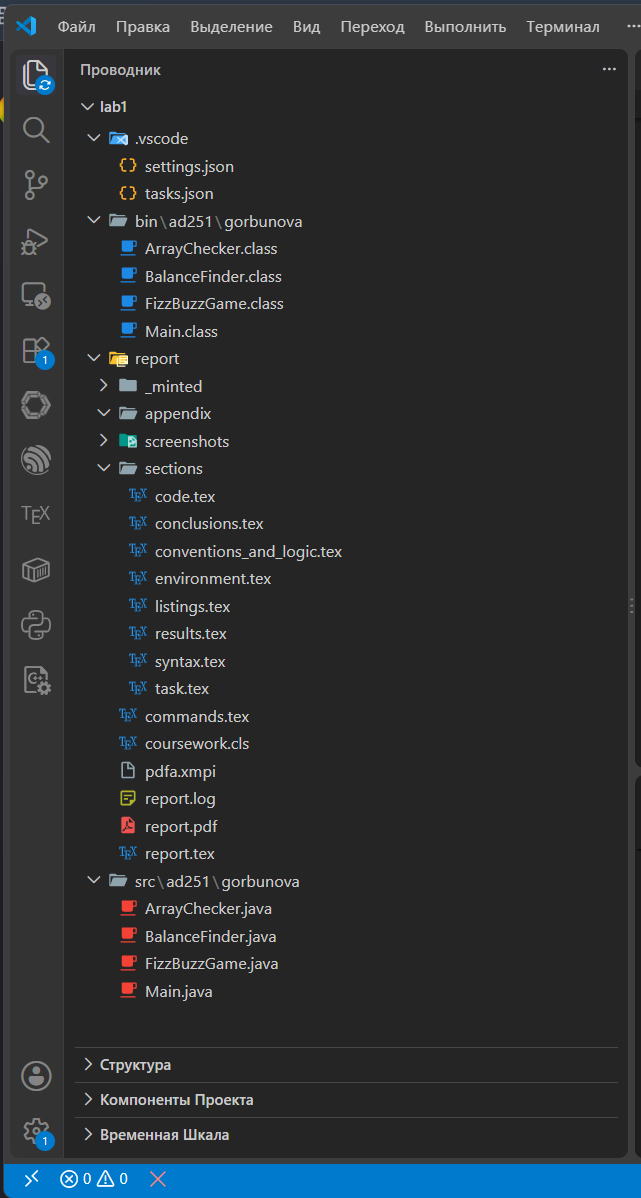
\includegraphics[width=0.45\textwidth]{screenshots/project_tree.png}
    \caption{Фізична структура каталогів проєкту із реалізацією базового пакету \texttt{ad251.gorbunova}}
    \label{fig:project_tree}
\end{figure}


